As seen in \S\ref{sec:panda_deployment}, PanDA Broker was  deployed on the DTNs
as Titan's worker nodes lack connectivity to the wide area network The lack of
pilot capabilities impacts both the efficiency and the flexibility of PanDA's
execution process. Pilots could improve efficiency by increasing throughput and
enabling greater backfill utilization. Further, pilots makes it easier to
support heterogeneous workloads.

As discussed in \S\ref{sec:panda_titan}, the absence of pilots imposes the
static coupling between MPI scripts submitted to the PBS batch system and
detector simulations. This makes the scheduling of multiple generations of
workload on the same PBS job impossible: Once a statically defined number of
detector simulations are packaged into a PBS job and this job is queued on
Titan, no further simulations can be added to that job. New simulations have to
be packaged into a new PBS job that needs to be submitted to Titan based upon
backfill availability.

The support of  multiple generations of workload would enable more efficient use
of the backfill availability of walltime. Currently, when a set of simulations
ends, the PBS job also ends, independent of whether more wall-time would still
be available. With a pilot, additional simulations could be executed  to utilize
all the available wall-time, while avoiding further job packaging and submission
overheads.

Multiple generations would also relax two assumptions of the current execution
model: knowing the number of simulations before submitting the MPI script, and
having a fixed number of events per simulation (100 at the moment). Pilots would
enable the scheduling of simulations independently from whether they were
available at the moment of submitting the pilot. Further, simulations with a
varying number of events could be scheduled on a pilot, depending on the amount
of remaining walltime and the distribution of execution time per event, as shown
in \S\ref{ssec:panda_titan}, Fig.~\ref{fig:100event- distrib}. These
capabilities would increase the efficiency of the PanDA Broker when there is a
large difference between the number of cores and walltime.

Pilots can offer a payload-independent scheduling interface while hiding the
mechanics of coordination and communication among multiple worker nodes. This
could eliminate the need for packaging payload into MPI scripts within the
broker, greatly simplifying the submission process. This simplification would
also enable the submission of different types of payload, without having to
develop a specific PBS script for each payload. The submission process would
also be MPI-independent, as MPI is used for coordination among multiple worker
nodes, not by the payload.

% -----------------------------------------------------------------------------
\subsection{Implementation}
\label{sec:arch}

The implementation of pilot capabilities within the current PanDA Broker require
quantification of the effective benefits that it could yield and, on the base of
this analysis, a dedicated engineering effort. We developed a prototype of a
pilot system capable of executing on Titan to study experimentally the
quantitative and qualitative benefits that it could bring to PanDA. We called
this prototype Next Generation Executor (NGE).

NGE is a runtime system to execute heterogeneous and dynamically determined
tasks that constitute workloads. Fig.~\ref{fig:arch-overview} illustrates its
current architecture as deployed on Titan: the two management modules (Pilot
and Unit) represent a simplified version of the PanDA Broker while the agent
module is the pilot submitted to Titan and executed on its worker nodes. The
communication between PanDA Broker and PanDA Server is abstracted away as it
is not immediately useful to evaluate the performance and capabilities of a
pilot on Titan.

\begin{figure}
  \centering
   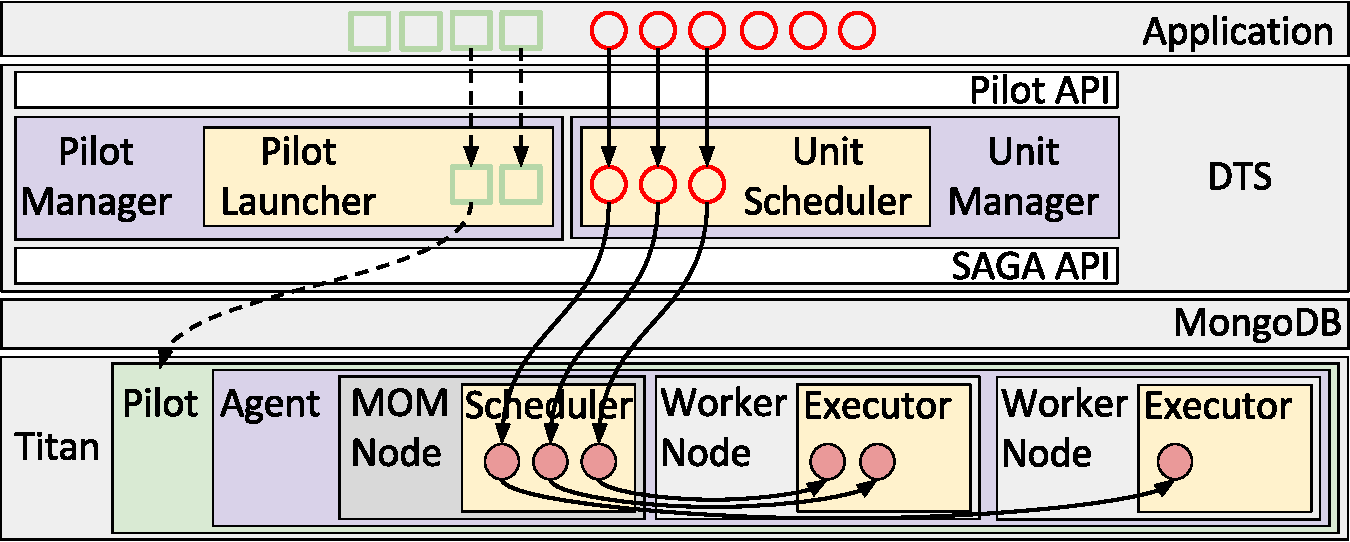
\includegraphics[width=\columnwidth]{figures/rp_architecture_compact_atlaswms_paper.pdf}
  \caption{NGE Architecture as deployed on Titan. The PilotManager and the
  UnitManager reside on one of Titan's DTN while the Agent is executed on
  Titan's worker nodes. Boxes color coding: gray for entities external to NGE,
  white for APIs, purple for NGE's modules, green for pilots, yellow for
  module's components.}
\label{fig:arch-overview}
\end{figure}

NGE exposes an API to describe workloads (Fig.~\ref{fig:arch-overview}, green
squares) and pilots (Fig.~\ref{fig:arch-overview}, red circles), and to
instantiate a PilotManager and a UnitManager.   The PilotManager submits
pilots to Titan's PBS  batch system via SAGA API (Fig.~\ref{fig:arch-overview}, dash arrow), as done by PanDA Broker to submit MPI scripts. Once
scheduled, the pilot's Agent is bootstrapped on Titan's MOM node and
the Agent's Executors on the on the worker
nodes, and the UnitManager schedules units to the Agent's Scheduler
(Fig.~\ref{fig:arch-overview}, solid arrow). The Agent's Scheduler schedules
the units on one or more Agent's Executor for execution. The Agent's executors
can manage one or more worker nodes, depending on performance evaluations. The
UnitManager and the Agent communicate via a database that is instantiated on
one of Titan's DTN so as to be reachable by both modules.

The NGE Agent uses the \emph{Open Run-Time Environment (ORTE)} for communication
and coordination of the execution of units. This environment is a critical
component of the OpenMPI implementation, developed to support distributed
high-performance computing applications operating in a heterogeneous
environment~\cite{castain05:_open_rte, cug-2016}.

ORTE provides a mechanism to create a \emph{``dynamic virtual machine''} (DVM)
that spans multiple nodes. The DVM transparently provides support for
interprocess communication, resource discovery and allocation, and process
launching across a variety of platforms. Libraries enable the interaction
between users and ORTE to enable the submission, monitoring and managing of
tasks, avoiding filesystem bottlenecks and race conditions with network sockets.
As a consequence, ORTE is able to minimize the system overhead while submitting
tasks.
